% TEMPLATE for Usenix papers, specifically to meet requirements of
%  USENIX '05
% originally a template for producing IEEE-format articles using LaTeX.
%   written by Matthew Ward, CS Department, Worcester Polytechnic Institute.
% adapted by David Beazley for his excellent SWIG paper in Proceedings,
%   Tcl 96
% turned into a smartass generic template by De Clarke, with thanks to
%   both the above pioneers
% use at your own risk.  Complaints to /dev/null.
% make it two column with no page numbering, default is 10 point

% Munged by Fred Douglis <douglis@research.att.com> 10/97 to separate
% the .sty file from the LaTeX source template, so that people can
% more easily include the .sty file into an existing document.  Also
% changed to more closely follow the style guidelines as represented
% by the Word sample file. 

% Note that since 2010, USENIX does not require endnotes. If you want
% foot of page notes, don't include the endnotes package in the 
% usepackage command, below.

% This version uses the latex2e styles, not the very ancient 2.09 stuff.
\documentclass[letterpaper,twocolumn,10pt]{article}
\usepackage{usenix,epsfig,endnotes,graphicx}
\usepackage{epstopdf, color}
% \DeclareGraphicsExtensions{.eps}

\begin{document}

%don't want date printed
\date{}

%make title bold and 14 pt font (Latex default is non-bold, 16 pt)

\title{\Large \bf BugBox : A Vulnerability Corpus for PHP Web Applications}


%for single author (just remove % characters)
\author{
{\rm Kent Wills}\\
Computer Science Department\\University of Maryland
\and
{\rm Gary Nilson}\\
Computer Science Department\\University of Maryland
% copy the following lines to add more authors
% \and
% {\rm Name}\\
%Name Institution
} % end author

\maketitle

% Use the following at camera-ready time to suppress page numbers.
% Comment it out when you first submit the paper for review.
\thispagestyle{empty}

\subsection*{Abstract}

This paper covers the motivation and architecture behind BugBox, an open-source collection and management framework for PHP web application vulnerabilities. It is recognized that obtaining an adequate vulnerability data-set is a major hurdle in empirical vulnerability research. Many studies suffer from using vulnerability data-sets that are too small and often not made publicly available [ref]. The purpose of BugBox is to fill this void, and in doing so encourage the quality and repeatability of results. The goal is to collect a large number of vulnerabilities across many applications, and make data available to the larger community. Example uses of BugBox include testing vulnerability indicators and metrics, developing vulnerability definition representations, testing intrusion detection systems, or creating demonstrations for training purposes. 

\section{Introduction}
\textcolor{red}{
(i.e. Introduction and Motivation)
[what is a corpus?
 what is empirical vulnerability research?
 what should a corpus contain?
 what cool things can BugBox do?]}

Building significant vulnerability corpus is not usually the main focus in vulnerability research.  Typically researchers want to develop their dataset quickly so that they can move on to more important work. Understanding why code is vulnerable can lead to automated techniques in preventing future vulnerabilities [more details on this]. An ideal vulnerability corpus would make it easy to explore each of these domains. We propose a framework based on common languages and tools, in order to manage and automate data collection in a way that is scalable to thousands of applications [specific, big claim].\par

The value of a corpus is mostly measured by the size and diversity of vulnerabilities and vulnerable applications represented. But quantity is not the only consideration. It is also useful that the collection be easy to maintain, and that vulnerability meta-data is encoded in way that fascilitates search, and automation in the experiments. Through the use of abstraction and encapsulation, the management of application, environment, and exploitation has been streamlined in BugBox. The design is intended to be make it practical to manage a large database of exploits, along with their target environments. To have these qualities the corpus must be much more than an exploit repository. For a given application, it should include the software in which a vulnerability exists, the software's dependancies, the configuration of the software in it's vulnerable state, exploit code that will trigger the security breach, and data that describes any distinguishing attributes of the bug. [define attributes futher]\par

Currently the framework is designed for PHP web applications. There are a number of factors for the decision to focus on collecting vulnerabilities only for PHP. Foremost, is that PHP remains on of the most popular languages for web applications [ref], and as has been reported by Top Cyber Security Risks to be a target for security threats [ref]. Web applications are subject to a rich variety of exploit types (such as XSS, CSRF, SQL injection, overflows, etc...) covering many actively maintained projects that are open source. In addition, popular vulnerability databases wuch as the National Vulnerability Database (NVD), Open Source Vulnerability Database (OSVDB), or the Exploit Database (EDB) have a large quantity of PHP application vulnerabilities. In addition, these databases often disclose enough details of the vulnerability that exploits can easily be written.\par
  
Key qualities:\\
 \begin{tabular}{ l }
   $\bullet$ Quantity of vulnerabilities\\
   $\bullet$ Diversity of applications\\
   $\bullet$ Automation of trace collection\\
   $\bullet$ Collaboration from other researchers\\
   $\bullet$ Ease of exploit implementation\\

 \end{tabular}
\\


\subsection{Empirical Vulnerability Research}


A key question in empirical vulnerability research is how to determine which functionality, or piece of code creates a vulnerable condition in a program. In studying this problem, sometimes referred to as \emph{vulnerability localization}, it is necessary to have a large quantity of structured data on which one can formulate and test hypotheses. Since potential approaches include vulnerability definitions based both static and dynamic analysis of the software, it is important that the corpus include both the vulnerable program's code, and some way to perform analysis as the system is compromised.\\


[many things with with references go here]\\

Demonstrate that BugBox ....\\
Should be x, should be y, and should be z.\\
Predicting which metrics  \\

Code inspection\\
Trace-based vulnerability definitions\\
System taint analysis\\
Selenium ... \\


``Vulnerability localization''

Characteristics:\\
 \begin{tabular} { l }
   -Collecting Vulnerable Application source code\\
   -Collecting vulnerability details\\
     a) line-based\\
     b) run-based\\
      i. trace-based\\
 \end{tabular}\\


\section{Framework}

The framework has five main components: web application store, testing environment, testing scripts, and host system. Figure 1 illustrates general structure of the corpus environment, with arrows showing lines of control or communication. The system was designed to be modular so that every component can be independently interchanged.\par
Currently BugBox is designed to work on any system compatable with the Debian GNU/Linux distribution. The key requirements are that the machine have sufficient storage (roughly 4 GB per OS environment, and 2 GB for the application, engine, and exploit sources [Confirm these #s]), that it should be capable of running a MySql serverer to host the various applicaiton databases, in addition to the Selenium Server (used in the exploit implementations). The system dependancies also include debootstrap for managing the application host environments, and the Advanced Packaging Tool (APT) [...]
   
At it's core, the orginization of the vulnerability engine is driven by the Python module and package system. The system breaks down into the following python modules:

 \begin{table}
 \begin{minipage}[b]{0.45\linewidth}
 \caption{Corpus Modules}
 \hline
 \begin{tabular}{ l }
   $\bullet$ corpus.Engine\\
   $\bullet$ corpus.Targets\\
   $\bullet$ corpus.Exploit\\
   $\bullet$ corpus.SeleniumDriver\\
 \end{tabular}
\end{minipage}
\end{table}


   {\bf Engine} drives the environment setup, tear-down, and exploition process. It contains most of the logic for doing work with exploits.
   {\bf Targets} module has as submodules each application and application plugin that are associated with an exploit.
   {\bf Exploit} is the superclass for each exploit in the corpus, defining interfaces and attributes that the engine uses to manage the environment and exploitation.
   {\bf SeleniumDriver} a wrapper class for the Slenium's Firefox web driver.


% you can also use the wonderful epsfig package...
%{\special{psfile = system_diagram.ps hscale = 50 vscale = 50}}
\begin{figure}[t]

\begin{center}
\begin{picture}(240, 195)(0,0) %(0,200)
\put(0,0){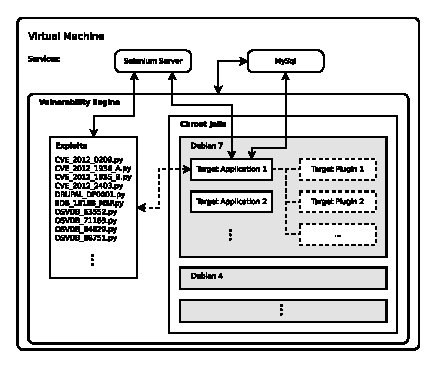
\includegraphics[scale=1.17]{system_diagram.eps}}
\end{picture}
\end{center}
\caption{System Diagram}
\end{figure}


\subsection{Vulnerability Engine}

\subsection{Environment}
\textcolor{red}{[Why we need different OS environments, how the corpus manages them]}

The corpus contains a main engine, written in python, to load a web application, gather traces, run exploits, and cleanup.  We provide an engine to abstract away the details of the setup process so that contributors can focus on creating new exploit scripts.  This separation accomplished two tasks, it makes developing for the corpus more approachable for programmers that want to contribute and provides a robust framework that can provide more of a challenge to seasoned programmers.

We use a virtual jail, the linux chroot environment.  Staging the application in the chroot environment provides locality, reproducibility, and stability.  

{\bf The web application remains local}.  Many applications, such as wordpress, have a MYSQL backend.  If we were to host the application on a different server or VM we would have to ensure that the MYSQL database is properly setup each time.  With the chroot environment, the process is simplified, we keep a MYSQL database outside of the CHROOT Jail in order to facilitate MYSQL access.  

{\bf Current tests are independent from future tests}.  We load a clean application into the chroot jail every time we wish to run a new test.  This ensures that there is no corruption of the original Web Application and provides reproducible results when testing.

{\bf The web application cannot contaminate our testing environment}.  If a web application crashes due to the malicious script, we can ensure that it does not crash our corpus environment, worst case the chroot is corrupted, and we can ensure that the crash cannot have un-intended side effects in our testing environment.  


\subsection{Target Module}
\textcolor{red}{The anatomy of a ``Target'' module}
\subsection{Exploit}

Management actions, recording commands
attributes,
\begin{verbatim} 
__init__()
exploit()
check() [not yet]
cleanup()
\end{verbatim}

{\tt \small
\begin{figure*}[!ht]
\begin{verbatim}
import corpus

class Exploit (corpus.Exploit):

    def __init__(self):
        corpus.Exploit.__init__(self, {
                'Name' :        "CVE_2012_2403",
                'Description' : "Creates a post containing a XSS payload.",
                'References' :  [['CVE','2012-2403'],
                                 ['OSVDB','81463']],
                'Target' :      "Wordpress 3.3.1",
                'Type' :        "XSS",
                'VulWikiPage' : "http://seamster.cs.umd.edu/CVE-2012-2403"
                })
        return
            
    def exploit(self):

        payload = "<a href=\"#\" title=\"XSS http://example.com/onmouseover"
                  "=eval(unescape(/%61%6c%65%72%74%28%31%29%3b%61%6c%65%72"
                  "%74%28%32%29%3b%61%6c%65%72%74%28%33%29%3b/.source))//\"
                  ">XSS</a>"

        driver = self.create_selenium_driver()
        driver.get("http://localhost/wordpress/?p=1")
        driver.find_element_by_id("author").clear()
        driver.find_element_by_id("author").send_keys("selenium script")
        driver.find_element_by_id("email").clear()
        driver.find_element_by_id("email").send_keys("selenium@python.org")
        driver.find_element_by_id("url").clear()
        driver.find_element_by_id("url").send_keys("www.python.org")
        driver.find_element_by_id("comment").clear()
        driver.find_element_by_id("comment").send_keys(payload)
        driver.find_element_by_id("submit").click()
        driver.cleanup()

        return

if __name__ == "__main__": # Exploit invoked from command-line
    engine = corpus.Engine(Exploit())
    engine.parse_args(sys.argv)
\end{verbatim}
\end{figure*}
}


\subsubsection{As a Standalone Application}

Each exploit is defined in it's own python file as a module. In Python, modules can either be imported from other modules, or executed directly from the command-line. The exploits written for BugBox take advantage of this property to give the researcher the option of writing scripts to do work on a set of exploits, or to invoke one exploit at a time. When run from the command-line, the supplied arguments are passed directly to the vulnerability engine, which supports the options shown below: 

{\tt \small
\begin{verbatim}
Usage: python OSVDB_89960.py [options]
Options:
    start:          Start exploit instance
    stop:           Stop exploit instance
    exploit:        Run the exploit
    check:          Check if the corresponding 
                    environment is running
    xdebug_on:      Turn on xdebug autotrace
    xdebug_off:     Turn off and collect 
                    xdebug autotrace
\end{verbatim}
}

\subsubsection{As a Python Module}
\textcolor{red}{
Scripting of experiments. corpus.Query [Work in progress] interface for using querys of exploit metadata to manage sets of exploits/environments. 
}


\subsubsection{Selenium Scripting}

We aim to gather code that is vulnerable.  We drastically can reduce the amount of computation needed by reducing the code size that needs to be analyzed through the use of past, found exploits.  

In order to better isolate vulnerable code, we create a selenium script in Python, replicating actions a user would take in performing an exploit on a web application.  While the script is running, we can have XDebug monitor the execution and output the final execution trace for the selenium script execution.  We can see future additions to this by turning XDebug on and off through cookie manipulation while the script is running, furthermore reducing the size of the vulnerable code.

By setting up the application loader engine, we are able to create concise python selenium scripts for data collection.  The following code shows how easy it is to run an automated exploit:

Pros:
-Ease of use, gret python bindings
-Uses browser's javascript engine
-Good for Demonstration/visualization

Cons:
-Not a necessary dependency, urrllib+cookielib would suffice
-requires SeleniumServer to run as a service on the host system
-Slower than crafting all requests directly
-Many times, we still need to use auxiliary libraries to send specially crafted requests anyway

[figure of a session hijack in a web-browser?]

We are restricted to web applications because of the use of selenium scripts in our corpus. [GJN ADD NOTES FROM JEFF's PAPER ON THIS]  


%{\tt \footnotesize
%\begin{verbatim}
%
%payload = "XSS PAYLOAD"
%
%driver = self.create_selenium_driver()
%
%driver.get("http://localhost/wordpress/?p=1")

%%Selenium Actions preceded by
%% driver.find_element_by_id
%("author").clear()
%("author").send_keys("selenium script")
%("email").clear()
%("email").send_keys("selenium@python.org")
%("url").clear()
%("url").send_keys("www.python.org")
%("comment").clear()
%("comment").send_keys(payload)
%("submit").click()
%
%\end{verbatim}
%}


\subsection{Trace Collection}
\textcolor{red}{
Stuff about interaction with XDebug.
}
XDebug is a feature-rich PHP debugger that can be used to easily collector traces enabling various run-time analyses.\par

\subsection{File Structure}

The file structure mimics the modularity of our corpus.  Currently we store backups of the Web Applications in the {\tt/backups} directory and the actual applications in the {\tt/packages} directory.  We store a separate backup in order to verify that the selenium scripts did not modify the Web Application in any way.  If the Web Application is corrupt, then we simply copy the web application from the backup folder to the package folder.  

Currently as simple incremental backup system is used to ensure that each chroot jail remains un-tainted. Periodically, an original instance of a chroot system will overwrite the 

Future implementations will store only the md5 hash of the program on the corpus server and the backups on an external server.  This will allow for a quick comparison followed by a remote copy if necessary.  This separation will ensure that backups will never be corrupted through use of the corpus.  

All the exploits that are available are located under the {\tt /scripts} folder.  While script is referenced as Selenium Script throughout the document, here scripts also include services such as: deploying the web application in the chroot jail, starting the trace collection, and running the script. All mounted chroot environments reside in {\tt /live\_systems}. 
\\\\
\textcolor{red}{
{\bf insert file system diagram}
}


\section{Scalability}
In order to create a system that can handle a growing amount of vulnerabilities that are independent from one another, we represent an exploit on an application through  Selenium scripts, as noted in the Framework section.  Selenium scripts allow us to perform operations on web applications without fear of working in an un-intended, compromised environment. 

\section{Use Cases}
By providing a corpus that explicitly logs the steps taken in accumulating the log files, we have more flexibility.  This flexibility can be seen with the following example:  
\\\\
{\tt Jon is told by his advisor that he needs to collect more trace data in order to get a proper sample size for his research.  John quickly creates a selenium script for the exploit he wants to collect and shows the advisor his results.  The advisor was generally happy with the trace data that he collected, but instead wanted him to do a slight modification to the exploit.  If Jon did not have the selenium script at hand, he would have to duplicate all of the work previously done.  Since he does have the script on hand, he can quickly make a change to the script and re-run in seconds versus hours.}
\\\\
While the above process is only shown in one iteration, most students know that this is not the case.  One hour of work can turn into a whole week of work without the proper framework in place.  The above situation also shows that the selenium script can be discussed with the professor to show validity of the data and provide talking points for how the exploit was applied.


\section{Acknowledgements}

Metasploit, undergraduate summer labor, etc..\\
Now we're going to cite somebody.  Watch for the cite tag.
Here it comes~.  The tilde character (\~{})
in the source means a non-breaking space.  This way, your reference will
always be attached to the word that preceded it, instead of going to the
next line.

\section{Future Development}
 \begin{description}
   \item[Distribution]
     \textcolor{red}{Virtual machine v.s. debian package. Pre-built chroot jails v.s. build scripts.
     i.e. size <--> setup proceess balance. Striking a balance between}
   \item[Services]
     \textcolor{red}{Why run Selenium/Mysql in VM vs a chroot jail?}
   \item[Isolating attack event]
     \textcolor{red}{(with xdebug manually/cookies/etc...)}   
   \item[Selenium driver and aux modules]
   Explore the possibility of a unified communication interface. This may be necessary in order to cleanly interact with xdebug with appropriate cookies set on a per-request basis (especially when modules other than Selenium are used for communication).
   \item[Payload standardization]
For each exploit currently in the corpus, there is no standard for the payload used in the attack. Since many studies may be sensitive to the payload type and encoding, it makes sense to provide the researcher with fine-grained control over this property. The Metasploit Framework has a very robust system for managing exploits along with their payloads and encodings, and can be a model for implementing this.
 \end{description}


\section{Conclusion}
\textcolor{red}{
Everything is great, we just need community involvement to mature the framework and to help write more exploits.
}
\section{Availability}
\textcolor{red}{
[Available as a 10 GB virtual machine and as a standalone debian package?]
}
\begin{center}
{\tt ftp://ftp.site.dom/pub/myname/Wonderful}
{\tt git://bugbox.github.com/blahblah}
\end{center}

\begin{center}
{\tt http://www.vulnerabilitywiki.com}
{\tt http://www.projecthomepage.com}
\end{center}

Now we get serious and fill in those references.  Remember you will
have to run latex twice on the document in order to resolve those
cite tags you met earlier.  This is where they get resolved.
We've preserved some real ones in addition to the template-speak.
After the bibliography you are DONE.

{\footnotesize \bibliographystyle{acm}
\bibliography{../common/bibliography}}


%\theendnotes

\end{document}







